Esta seção apresenta os resultados experimentais obtidos a partir da aplicação da metodologia descrita na Seção~\ref{sec:method}. O objetivo é validar as abordagens propostas e analisar o comportamento do modelo sob diferentes condições. Inicialmente, são descritos o ambiente computacional e os hiperparâmetros utilizados no treinamento do modelo base. Em seguida, investiga-se o impacto da etapa de remoção de ruído e das diferentes formulações da função de perda no desempenho preditivo. Por fim, é conduzido um estudo comparativo abrangente entre diferentes arquiteturas EfficientNet, avaliando o trade-off entre custo computacional e efetividade.

\subsection{Ambiente Experimental}

Os experimentos foram conduzidos em uma estação de trabalho Linux equipada com um processador AMD Ryzen 5 5600X, 32 GB de memória RAM DDR4 (3200 MHz) e uma GPU NVIDIA GeForce RTX 3060 (12 GB de VRAM), dedicada à aceleração do treinamento dos modelos de aprendizado profundo. O desenvolvimento foi realizado em Python utilizando o framework PyTorch integrado ao CUDA 12.8. Para o processamento de imagens histopatológicas, foi utilizada a biblioteca OpenSlide para leitura das imagens e extração de patches. As métricas de avaliação foram calculadas com o scikit-learn e as análises visuais foram geradas com o Matplotlib.

\subsection{Configuração de Hiperparâmetros}

A etapa inicial da experimentação consistiu em uma busca em grade (\textit{grid search}) para identificar a configuração de hiperparâmetros que maximizasse a convergência e a generalização do modelo base, mitigando o risco de overfitting. Os valores explorados e a configuração final selecionada estão resumidos na Tabela~\ref{tab:hiperparametros_gridsearch}. Essa configuração ótima foi definida como padrão e mantida constante nos experimentos subsequentes para garantir a comparabilidade dos resultados.

A taxa de aprendizado inicial definida como $3\times10^{-4}$, em conjunto com o otimizador Adam, proporcionou a melhor estabilidade durante a minimização da função de perda (BCE). Para o \textit{fine-tuning}, o descongelamento das últimas 150 camadas da rede apresentou o melhor equilíbrio. Além disso, uma camada de \textit{dropout} com probabilidade de retenção de 0.4 mostrou-se a estratégia de regularização mais eficaz. O tamanho do batch foi limitado a duas amostras devido às restrições de memória da GPU. Para mitigar flutuações nas atualizações de gradiente causadas pelo pequeno batch size, o treinamento foi configurado para até 50 épocas, utilizando \textit{early stopping} com paciência de 7 épocas sem melhoria na métrica de validação.

Para mitigar o tamanho limitado do conjunto de dados e melhorar a generalização, foi aplicada \textit{data augmentation} durante o treinamento utilizando a biblioteca Albumentations. As transformações incluem transposições aleatórias, flips horizontais e verticais, aumentando a variabilidade das amostras e reduzindo o overfitting.

\begin{table}[htb]
	\centering
	\begin{tabular}{lll}
		\toprule
		\textbf{Parâmetro} & \textbf{Valores avaliados} & \textbf{Valor selecionado} \\
		\midrule
		Taxa de aprendizado & $3\times10^{-4}$, $3\times10^{-3}$, $1\times10^{-4}$ & $3\times10^{-4}$ \\
		Número de épocas & 50 & 50 \\
		Camadas descongeladas & 100, 150 & 150 \\
		\textit{Dropout} & 0.4, 0.5, 0.6 & 0.4 \\
		Tamanho do batch & 2 & 2 \\
		Função de perda & BCE & BCE \\
		Otimizador & Adam & Adam \\
		\bottomrule
	\end{tabular}
	\caption{Hiperparâmetros avaliados e configuração selecionada para os experimentos.}
	\label{tab:hiperparametros_gridsearch}
\end{table}

\subsection{Impacto da Filtragem de Ruído e das Funções de Perda}

Com o conjunto ótimo de hiperparâmetros definido, o modelo base foi treinado utilizando a arquitetura EfficientNet-B0 e a função de perda BCE. Esse modelo alcançou uma acurácia de 0.592 e um coeficiente Kappa de 0.826. No contexto da classificação ISUP, esse valor é considerado altamente satisfatório e competitivo, superando significativamente a variabilidade entre patologistas reportada na literatura.

A etapa de filtragem baseada em entropia identificou 903 amostras (10\%) com maior incerteza. A remoção parcial (~20\%) dessas amostras resultou em melhora de desempenho, como mostrado na Figura~\ref{fig:acckappa}.

\begin{figure}[H]
	\centering
	
\includegraphics[width=1\linewidth]{images/acc_kappa}
	\caption{Desempenho sob diferentes níveis de remoção de ruído.}
	\label{fig:acckappa}
\end{figure}

\begin{figure}[H]
	\centering
	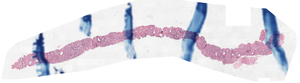
\includegraphics[width=0.7\linewidth]{images/max_entropy}
	\caption{Imagem identificada como ruidosa pelo método.}
	\label{fig:maxentropy}
\end{figure}

A substituição da BCE pela função ordinal aumentou o Kappa para 0.851, concentrando erros entre classes adjacentes, comportamento desejável clinicamente.

\begin{figure}[htb]
	\centering
	
\includegraphics[width=1\linewidth]{images/confusion_matrices_baseline}
	\caption{Matrizes de confusão (BCE vs ordinal).}
	\label{fig:confusionmatricesbaseline}
\end{figure}

A função híbrida (Ordinal + Focal) alcançou o melhor desempenho global:

\begin{table}[!htb]
	\centering
	\resizebox{1.2\textwidth}{!}{
		\begin{tabular}{lcccc}
			\toprule
			Configuração & Kappa & Acurácia & F1 & Precisão \\
			\midrule
			BCE & 0.826 & 0.592 & 0.537 & 0.551 \\
			BCE + Ruído & 0.833 & 0.638 & 0.572 & 0.584 \\
			Ordinal & 0.851 & 0.608 & 0.559 & 0.585 \\
			\textbf{Ordinal + Focal} & \textbf{0.857} & \textbf{0.669} & \textbf{0.612} & \textbf{0.628} \\
			\bottomrule
	\end{tabular}}
	\caption{Impacto das estratégias propostas}
	\label{tab:impacto_loss_expandido}
\end{table}

\begin{figure}[htbp]
	\centering
	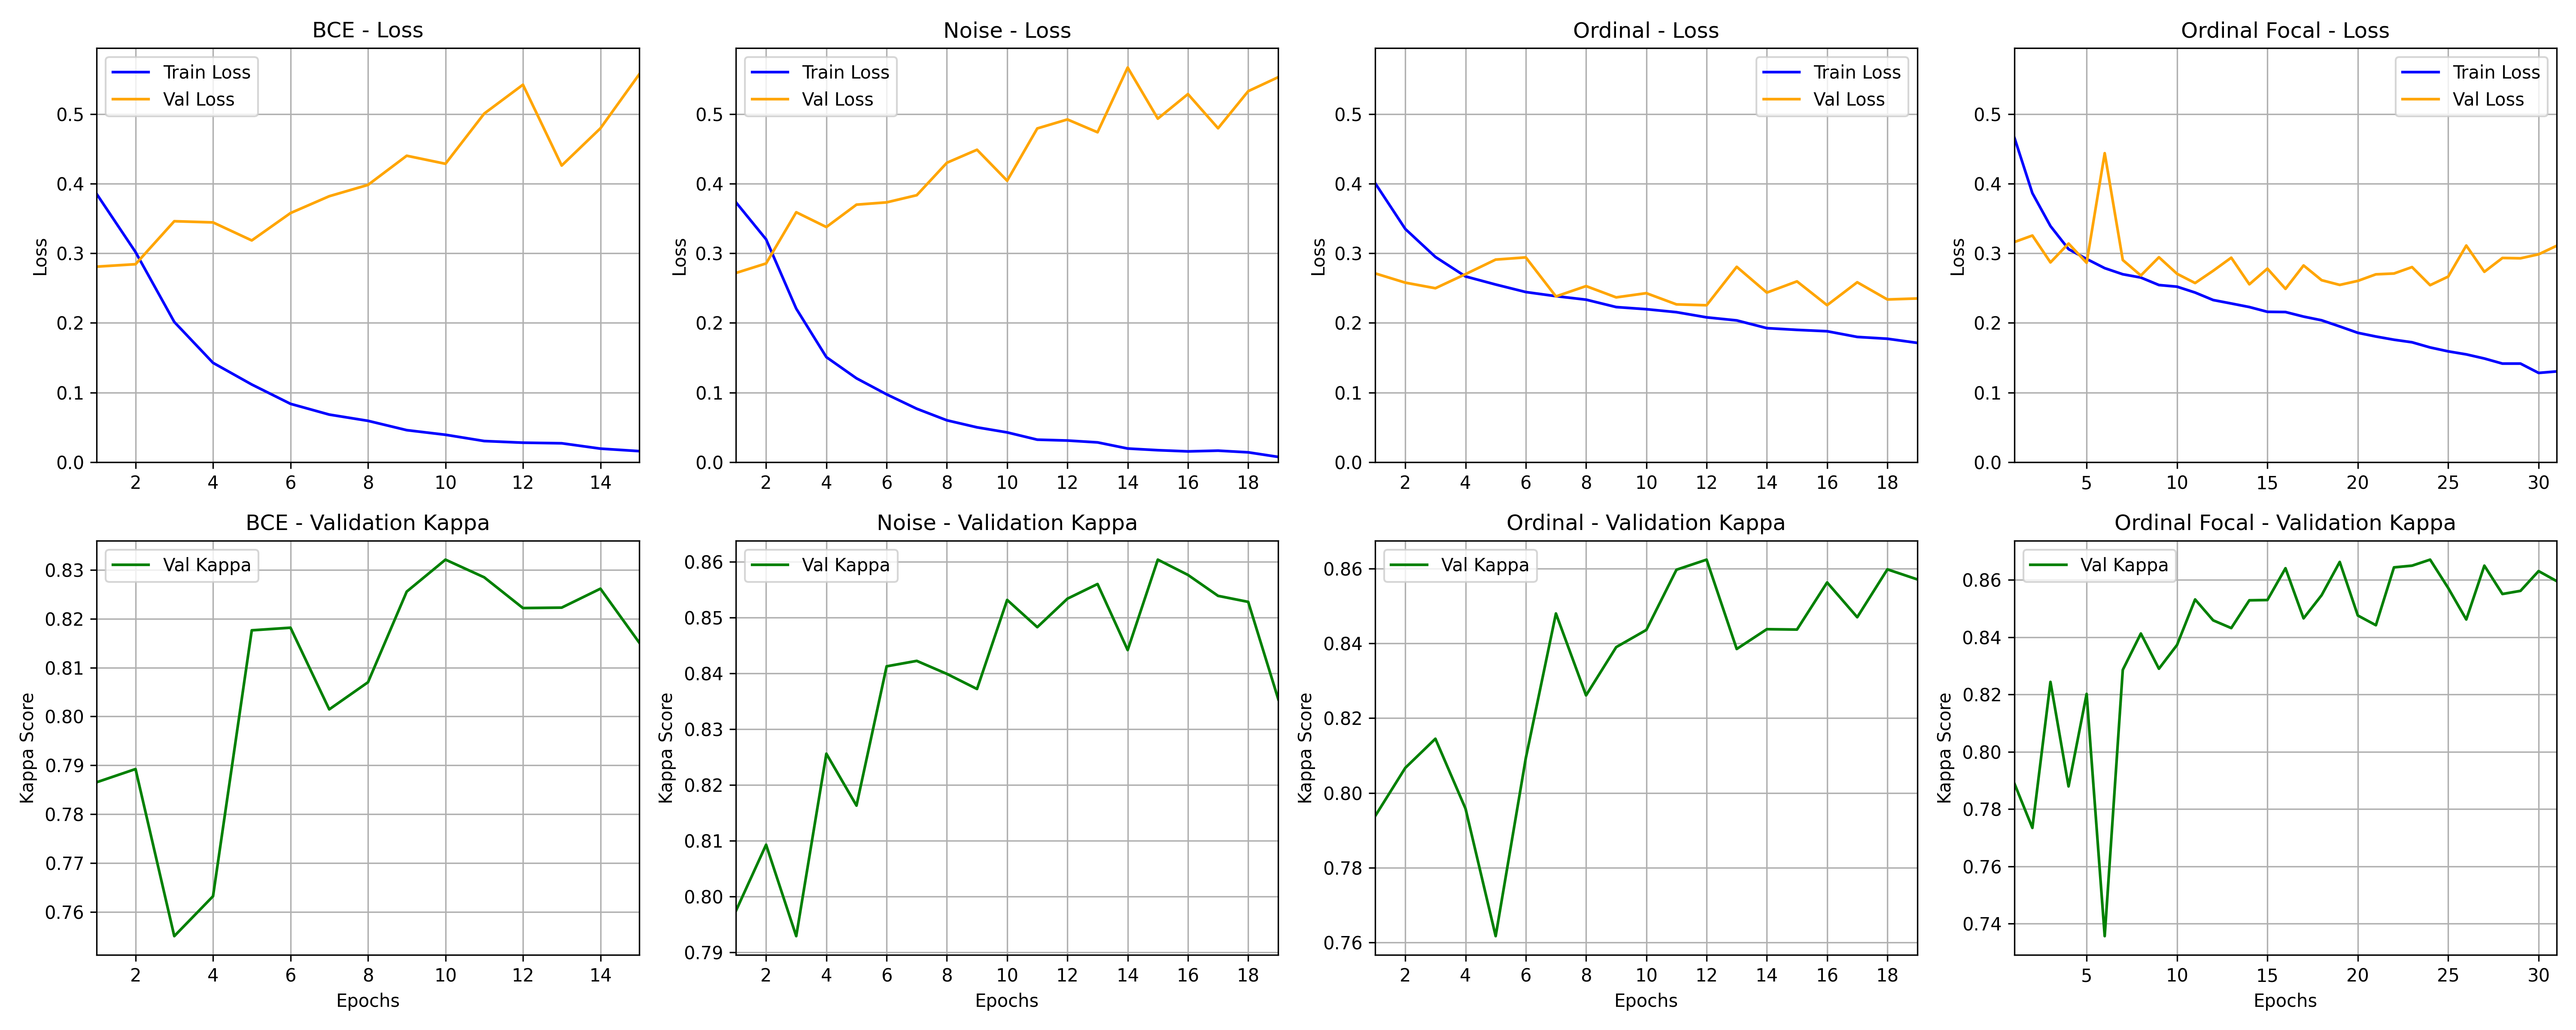
\includegraphics[width=1.2\linewidth]{images/plot_loss_kappa_4models.png}
	\caption{Curvas de loss e kappa}
	\label{fig:training_curves}
\end{figure}

\begin{figure}[!htb]
	\centering
	\subfloat{
		
\includegraphics[width=0.47\textwidth]{images/cm_ordinal.png}
	}
	\subfloat{
		
\includegraphics[width=0.47\textwidth]{images/cm_ordinal_focal.png}
	}
	\caption{Matrizes de confusão normalizadas}
	\label{fig:cm_ordinal_focal}
\end{figure}

\subsection{Comparação entre Arquiteturas EfficientNet}

A EfficientNet-B0 apresentou melhor desempenho geral:

\begin{table}[!htb]
	\centering
	\begin{tabular}{lcccc}
		\toprule
		Arquitetura & Kappa & Acurácia & F1 & Precisão \\
		\midrule
		B0 & \textbf{0.857} & \textbf{0.669} & \textbf{0.612} & \textbf{0.628} \\
		B3 & 0.849 & 0.661 & 0.555 & 0.605 \\
		B7 & 0.842 & 0.654 & 0.556 & 0.561 \\
		\bottomrule
	\end{tabular}
	\caption{Comparação entre arquiteturas}
	\label{tab:comparacao_arquiteturas}
\end{table}

\begin{figure}[htbp]
	\centering
	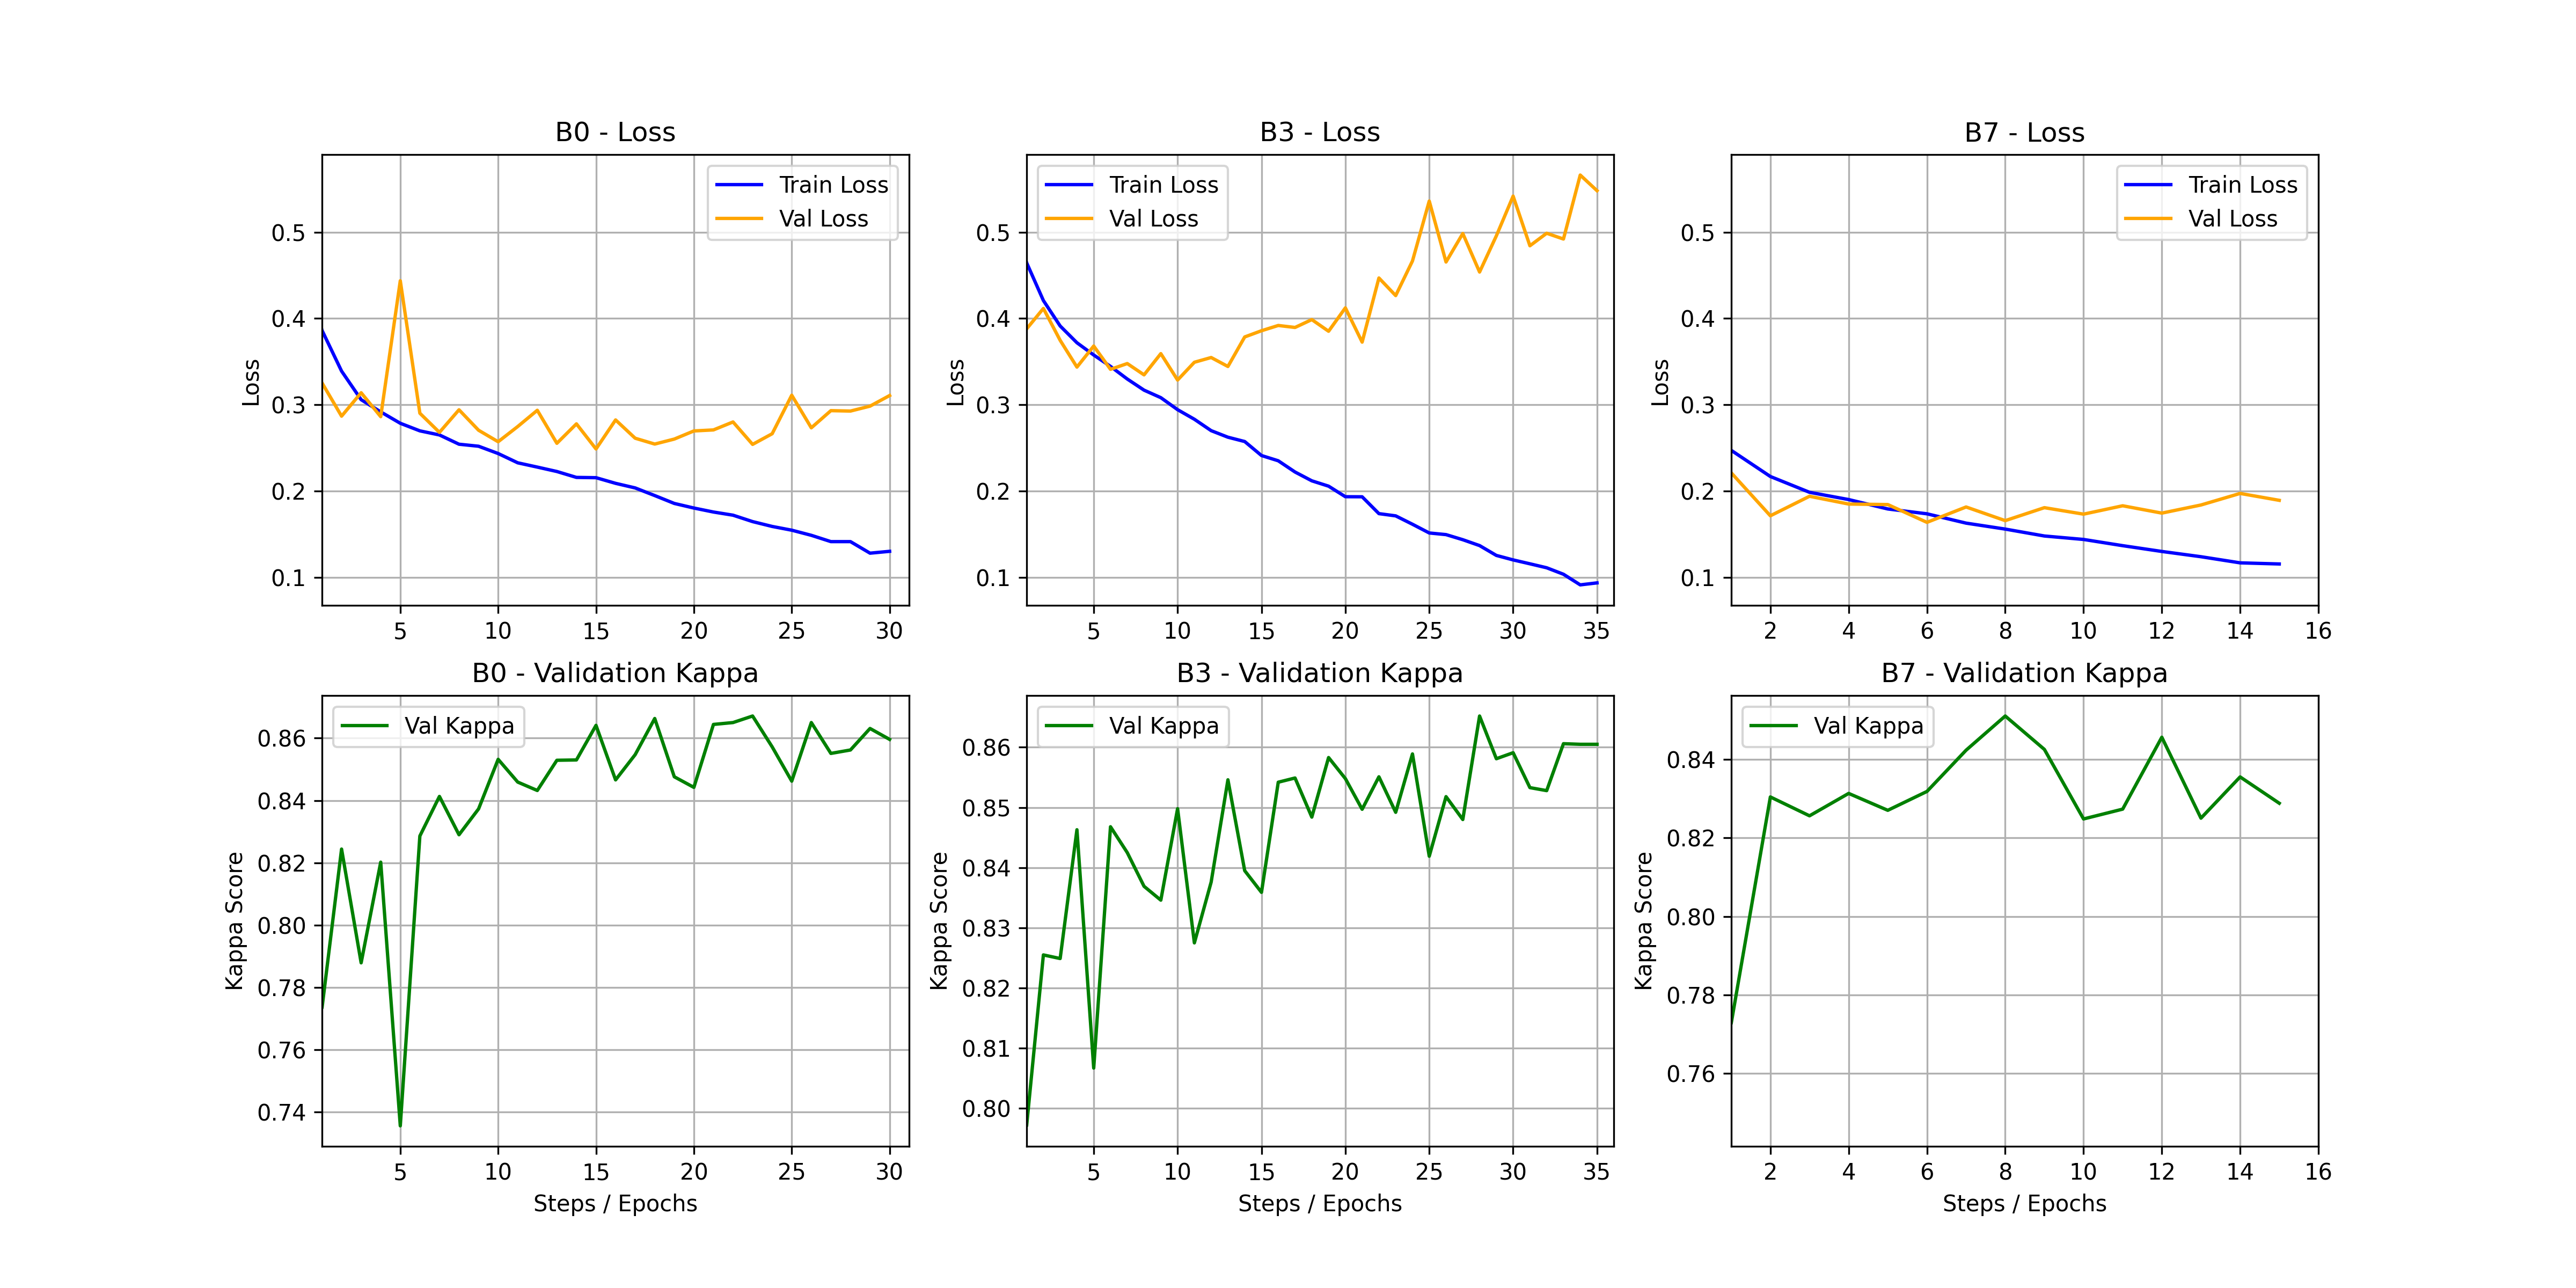
\includegraphics[width=1.5\linewidth]{images/plot_loss_kappa}
	\caption{Curvas de treinamento}
	\label{fig:plotlosskappa}
\end{figure}

Os resultados mostram que hiperparâmetros não escalam linearmente com a profundidade do modelo, reforçando a necessidade de ajustes específicos por arquitetura.